\chapter{Identifying the Environment Model }
\begin{itemize}
	\item What is the importance of model identification?
    \item How to identify?
    \item What's the data availability and quality?
    \item Are there differences for identifying different kind of models?
    \item What are the challenges?
\end{itemize}
Physiological models are developed to represent certain physiological condition in general, or the physiological condition of a specific patient. Therefore the structure of the model and corresponding parameters have to be identified. These information can be obtained from physiological data, which are from: 1) data collected during physiological procedures, and/or 2) physiological literature in which physiological data are analyzed and summarized. Due to limitation on the interactions with the patient, the availability and quality of physiological data are generally bad and there are generally not enough information to identify all the parameters in the model. It is essential to choose the right level of abstraction so that the model is identifiable (to a large extend). Having physiological correspondence for the model structure and parameters can also simplify the identification process. The rigorousness of the model identification step is also an important factor for the validity of the model. 

In the following sections, we briefly discuss our model identification effort for heart models used in two closed-loop verification applications, and their corresponding challenges. 
\begin{figure}[!t]
\centering
		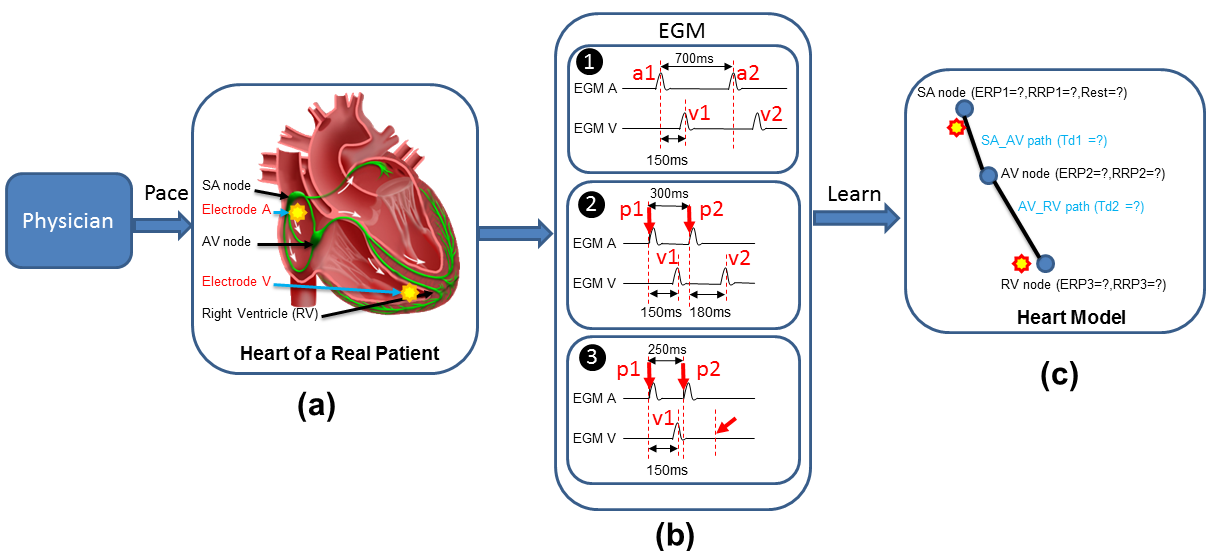
\includegraphics[width=0.9  \textwidth]{figs/modelID.png}
		
%\vspace{-10pt}
\caption{\small (a) The illustration of the probe locations. (b) 3 pacing sequences with different timing outcomes. (c) The heart model with undecided parameters}
\label{fig:modelID}
%\vspace{-15pt}
\end{figure} 

\section{Heart Model Identification for Closed-loop Simulation}
In closed-loop simulation, a heart model should be identified to represent a specific patient under certain heart condition. The constraints for model parameters can be obtained from patient data during \emph{ElectroPhysiological (EP) Testing}. During EP testing, the physicians deliver electrical pacing sequence from electrodes placed inside the patient's heart while extracting timing parameters from observed pattern and timing of electrical events. Since the goal for any EP testing procedure is not to determine all the timing parameters for a patient, the amount of parameters that can be identified from the patient data is limited.    

\figref{modelID} illustrates how timing parameters can be extracted during an EP testing procedure. \figref{modelID}.a shows a setup with two electrodes placed in the right atrium and right ventricle of the heart respectively. EGM signals can be measured from these two electrodes (\figref{modelID}.b). The physician can also apply pacing sequences through the electrodes which can trigger different response from the patient's heart. \figref{modelID}.c shows a heart model structure with unknown parameter values. By analyzing the \emph{timing} and \emph{pattern} of the EGM signals we can extract constraints on the parameters. In EGM sequence 1, the interval between two intrinsic activations $a1$ and $a2$ in EGM A is 700ms, so we have:
$$ERP1+RRP1+Rest=700ms$$
The interval between $a1$ and $v1$ is 150ms, so we have:
$$Td1+Td2=150ms$$
In EGM sequence 2, the pacing interval from Electrode A is 300ms. By observing that the interval between $p1-v1$ is less than the interval between $p2-v2$, we know that $p2$ arrives during the RRP period of the AV node. So we have:
$$ERP1+RRP1\leq 300ms$$
In EGM sequence 3, the pacing interval is further reduced to 250ms. There is no $v2$ corresponding to $p2$, indicating $p2$ arrives during the ERP period of the AV node. So we have:
$$ERP1\leq 250ms$$
We can see that each experiment provides certain time constraints for model parameters. By systematically conducting experiments certain model parameters can be uniquely identified within a relatively small range. However even with simplified model structure like the one in the example, not all model parameters can be uniquely identified due to limited number of electrodes and limited number of experiments during a real procedure.






\section{Heart Model Identification in Closed-loop Model Checking}
In model checking, the heart models in general have simple structure and less parameters due to non-deterministic abstraction. The heart models are developed in consistent with Electrophysiology terminologies, thus each node and path automata and their timing parameters have physiological correspondence which can be found in literature (\figref{intervals}). The range for non-deterministic parameters directly correspond to the range for possible values of corresponding physiological parameters. Therefore model identification for model checking is much simpler. 

\begin{figure}[!t]
\centering
		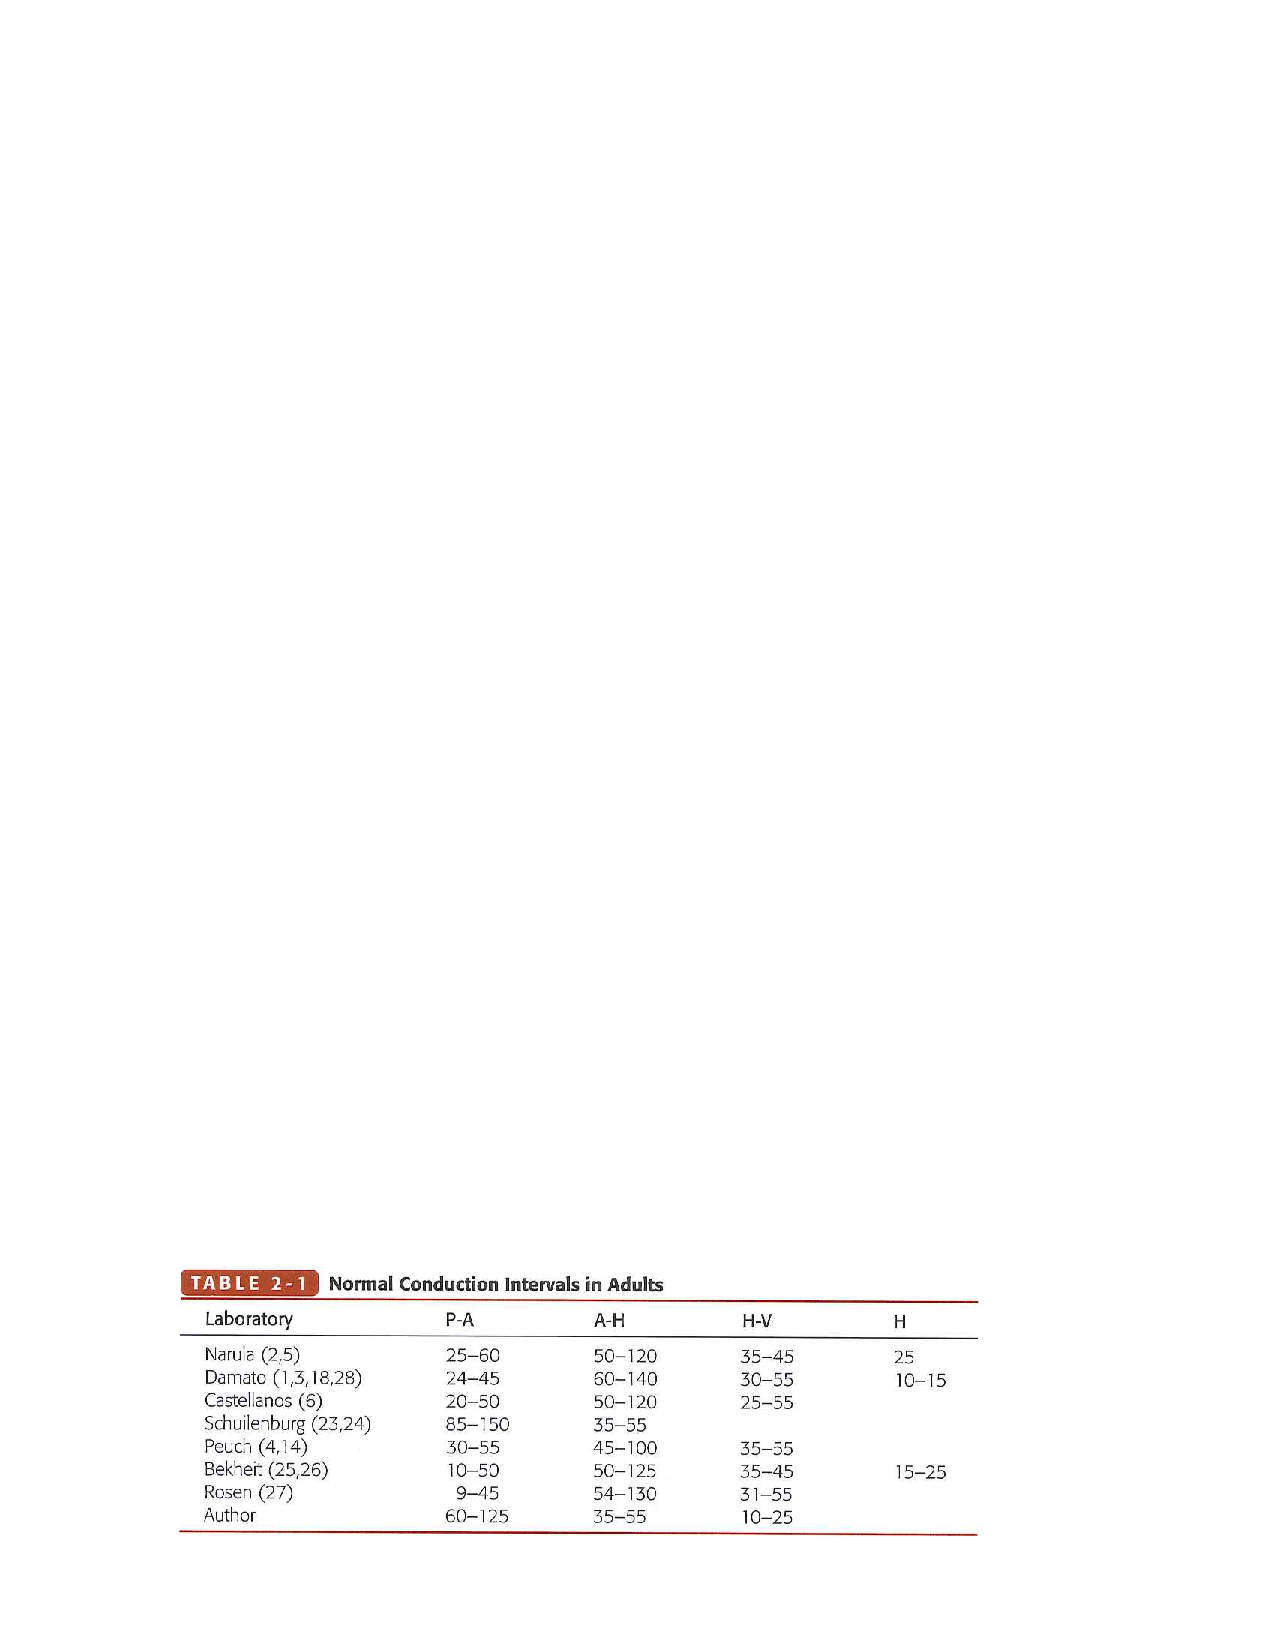
\includegraphics[width=0.8\textwidth]{figs/intervals.pdf}
		
%\vspace{-10pt}
\caption{\small Timing intervals measured during clinical studies \cite{josephson}}
\label{fig:intervals}
%\vspace{-15pt}
\end{figure} 







\chapter{Validating the Environment Model}
\begin{itemize}
	\item What are the different methods to validate physiological models?
    \item How much confidence can these validation provide?
\end{itemize}
The validity of the environment models affects the validity of the closed-loop verification results. Since models are always approximations of the actual environment, there is always discrepancies between the model and the actual patient (group). The challenge then is to evaluate the amount of safety guarantee that model-based closed-loop verification can provide. For the two closed-loop verification applications, the validity metric for the environment model is slightly different: in closed-loop model checking, the model's \textbf{coverage} on environmental behaviors is more important, while in closed-loop simulation, the \textbf{accuracy} of the model is more important. In this chapter we use our heart models as example to demonstrate several validation procedures that can improve the validity of the environment model.

\section{Validating Models for Closed-loop Simulation}
A physiological model is considered valid to be used in closed-loop simulation if 1) it is capable of generating the same output as the patient given the same input; 2) it is general enough to represent other patient with similar condition by adjusting its parameters. The second point is to ensure that the model successfully captures the underlying mechanism instead of over-fitting the data. In the following example we demonstrate the capability of our heart models to model certain heart conditions according to the mechanism described in physiological literature, and the model exhibits expected output given the proposed inputs.

%To use a physiological model for closed-loop simulation, there are two levels of validity: 1) model a patient with certain heart condition, 2) model a \em ph{specific} patient with certain heart condition. Level 1 validity ensures that the model successfully models the underlying mechanism of the heart condition, while level 2 validity guarantees the capability of the model to generate same data as the corresponding patient given the same input. Note that satisfying level 2 without satisfying level 1 may result in over-fitting.
\begin{figure}[!t]
\centering
		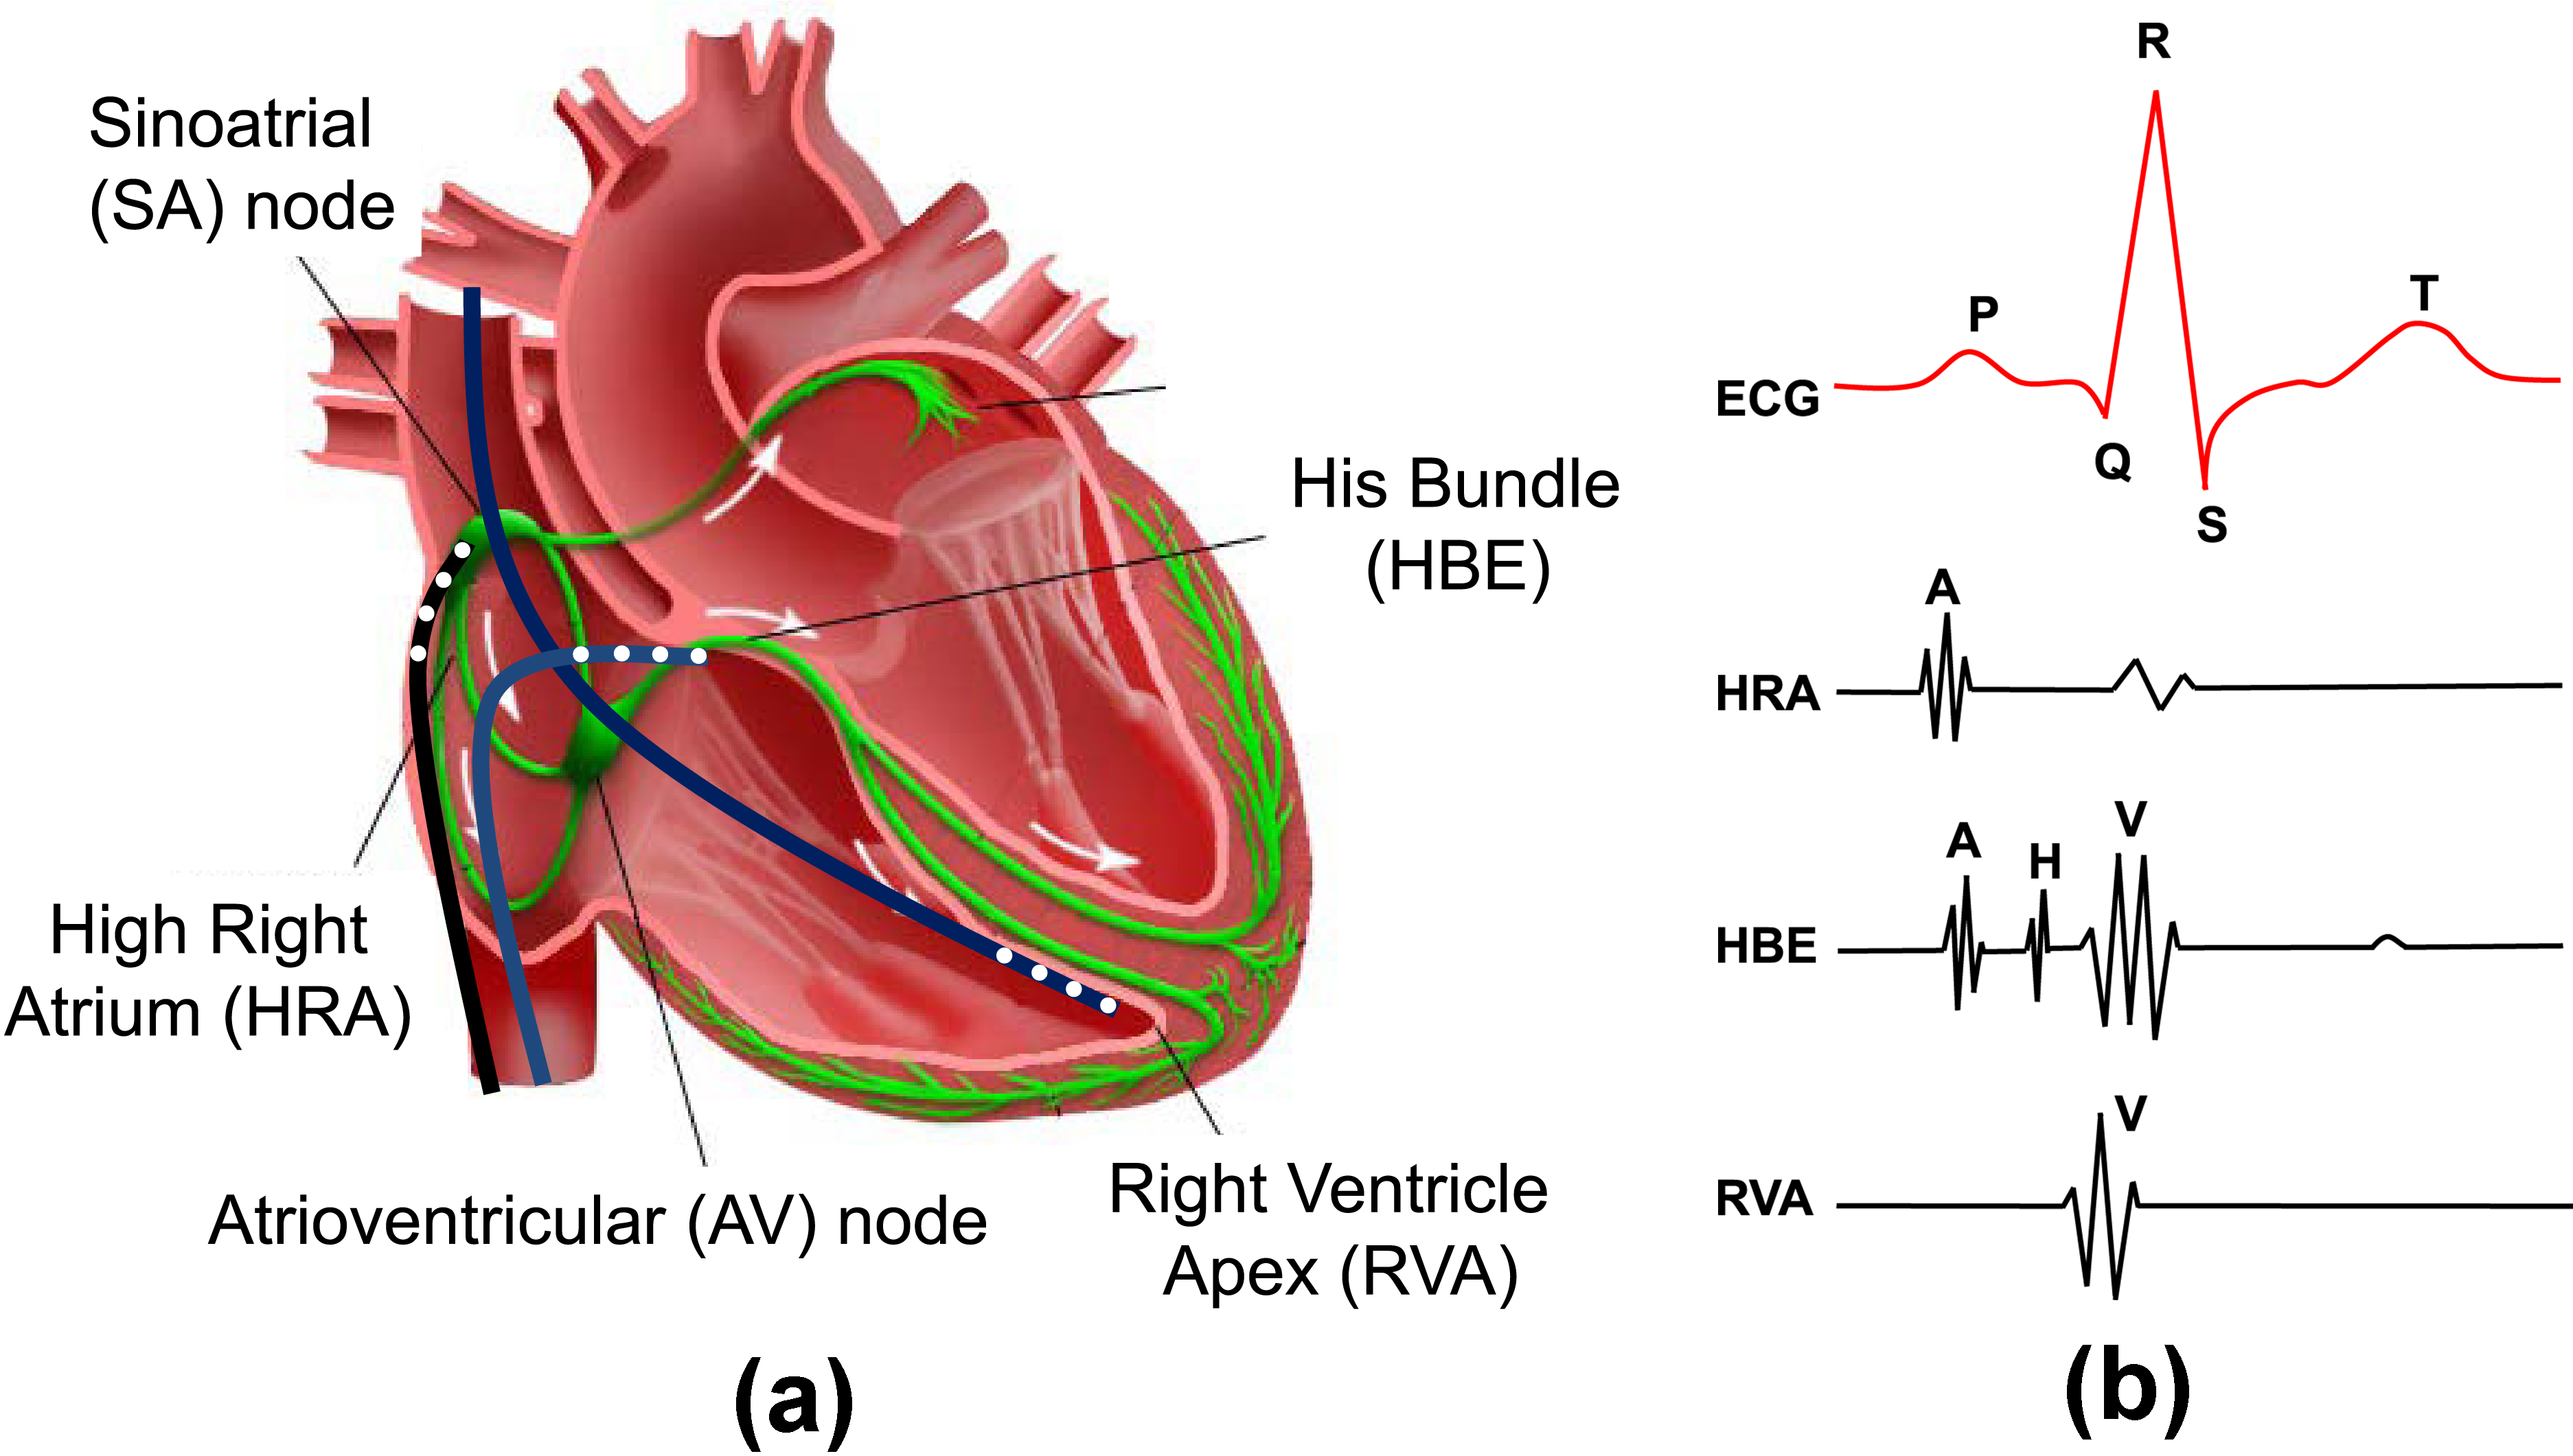
\includegraphics[width=0.9  \textwidth]{figs/probes.png}
		
%\vspace{-10pt}
\caption{\small (a) Probe locations for a general EP testing procedure. (b) EGM signals measured from the probes}
\label{fig:egm}
%\vspace{-15pt}
\end{figure} 

During an EP testing procedure, the physician place catheters inside the patient's heart to observe local electrical activities from different locations of the heart. The His bundle catheter (HBE) is particularly important when evaluating the atria-to-ventricle conduction path (\figref{egm}). For each A to V conduction there are 3 impulses which correspond to atrial contraction (A), His bundle activation (H) and ventricular activation (V).  In this case study, two pacing signals $a1$ and $a2$ are delivered to the heart from the HRA catheter. By gradually decreasing the pacing interval in each test, certain tissue along the A-V conduction path will be activated during its refractory period, thus affecting the conduction delay further down the conduction path and change the intervals between the impulses. \figref{book_1}.a shows the relation between pacing interval ($a1$-$a2$) and corresponding intervals between A, H and V impulses. On the left side it shows that interval $H_1-H_2$ and $V_1-V_2$ decrease but remain equal as the pacing interval decreases, indicating the tissue with the longest refractory period along the path is not between the His Bundle and the ventricles. When the pacing interval decreases to 350ms both intervals increases, indicating that the RRP of certain tissue has been reached and the tissue is between the atria and the His bundle. On the right it shows that the $A_2-H_2$ interval increases as the pacing interval decreases, which further proves the hypothesis that the AV node, which is between the atria and the His bundle has the longest refractory period along the A-V conduction path. We configured our heart model such that the AV node has the longest refractory period and performed the same study by decreasing the pacing interval. The result shows the exact same trend as the real patient (\figref{type_1}).
\begin{figure*}[!t]
\centering
		\subfigure 	[\small (~\cite{josephson})] 
		{
		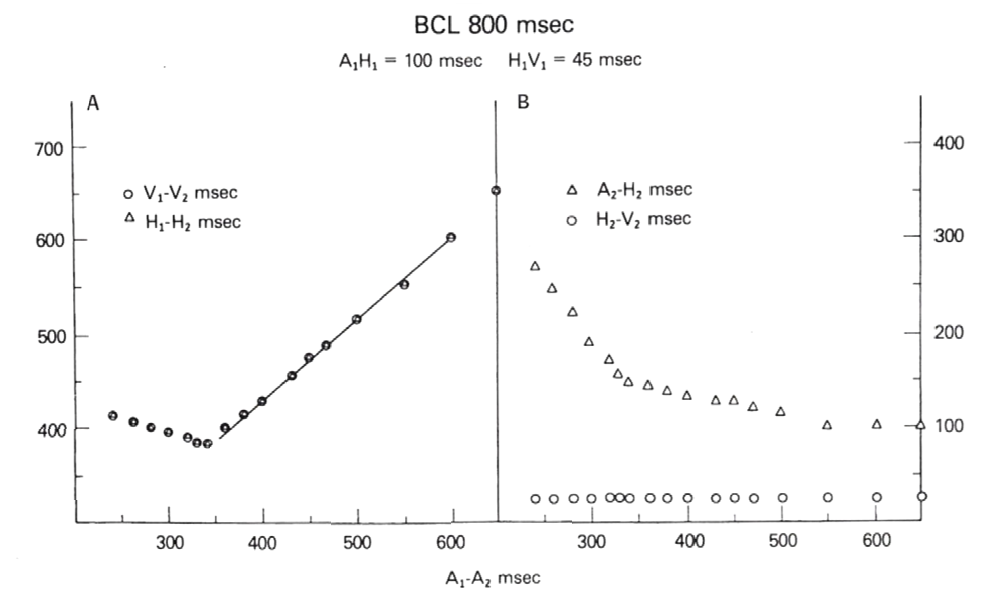
\includegraphics[width=0.5\textwidth]{figs/book_1.png}
		\label{fig:book_1}
		} 
		\subfigure [\small ] 
		{	
			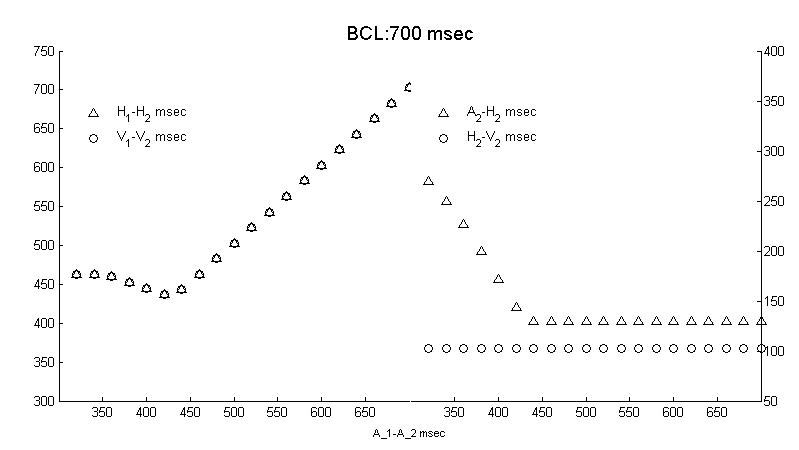
\includegraphics[width=0.45\textwidth]{figs/type_1.png} 
			\label{fig:type_1}
		}
\label{fig:Case_1}
%\vspace{-5pt}
\caption{\small Key interval values when the coupling interval shortens for (a) a real patient and (b) in VHM simulation ~\cite{vhm_ecrts10}.}
%\vspace{-15pt}
\end{figure*} 


% \begin{figure}[\b]
% 	\center
% 	\vspace{-20pt}
% %	\includegraphics[width=0.49\textwidth]{figs/AV_reentry_circuit.pdf}
% 	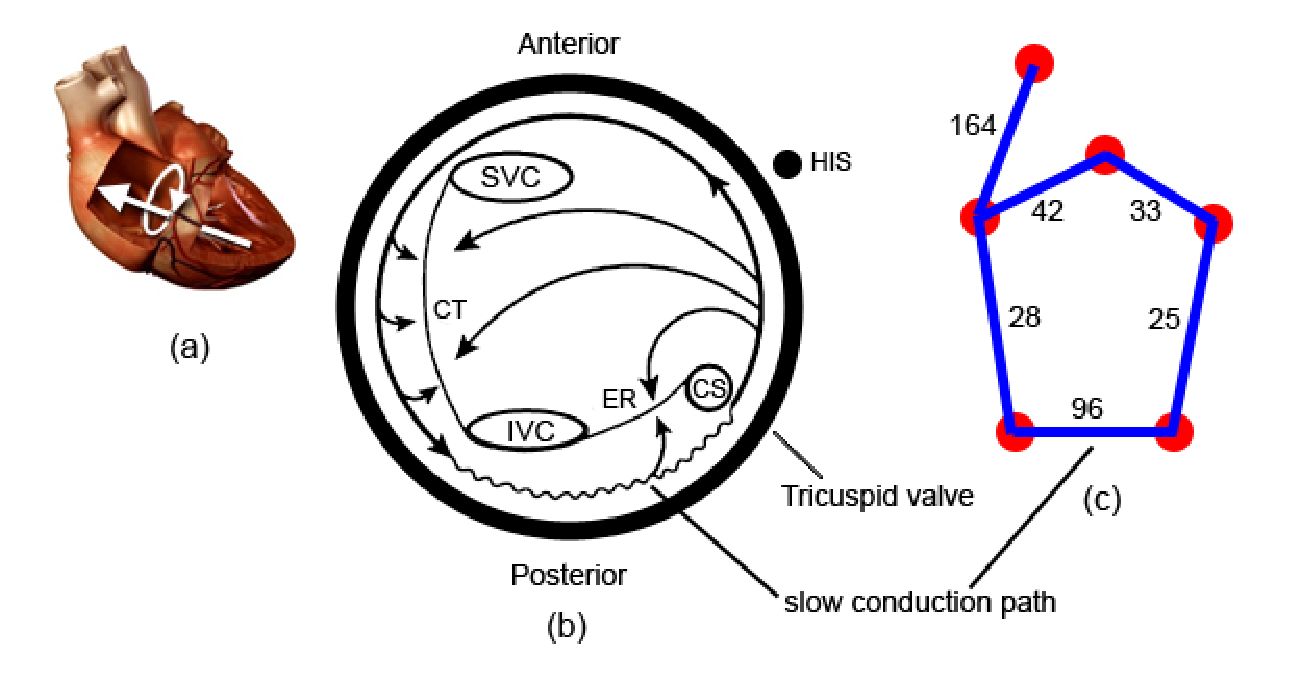
\includegraphics[width=0.5\textwidth]{figs/AFL_circuit.pdf}
% 	\center
% 	\vspace{-15pt}
% 	\caption{(a) The straight arrow shows the view of the AFL circuit from the right ventricle through the tricuspid valve into the right atrium, while the curved area shows the direction of conduction. (b) The circuit is bounded by the eustachian ridge (ER), connecting the  inferior vena cava (IVC) and the coronary sinus (CS), as well as the crista terminalis (CT), connecting the superior vena cava (SVC) and the IVC. The wavy line shows slow conduction through the CTI, bounded by the ER and the tricuspid valve (\emph{Adapted from} \cite{AFL_diag}). (c) The AFL circuit in the VHM extrapolates nodes and paths from the true physiology. The numbers show the values of conduction timers in the paths, with corresponding slow conduction path on the bottom.}
% 	\label{fig:AFL}
% \end{figure}

\section{Validate Models for Closed-loop Model Checking}
In model checking, a lot of complex dynamics of the environment are abstracted so that the environment model covers large number of environmental behaviors using non-determinism. The validity of the model can be provided by a valid initial model and a rigorous abstraction processes. In \cite{STTT13}, we started with a valid model and by applying different abstraction steps we were able to generate a series of non-deterministic heart models. Between each abstraction levels, the heart models satisfy a timed simulation relationship (\cite{simulation}) which is described below. The timed simulation guarantees all behaviors are covered in the mode abstract model.

For two timed automata $T^1=\left\langle S^1,S_0^1,\Sigma^1,X^1,inv^1,E^1\right\rangle$ and $T^2=\left\langle S^2,S_0^2,\Sigma^2,X^2,inv^2,E^2\right\rangle$, a timed simulation relation is a binary relation $\textsf{sim}\subseteq \Omega^1\times \Omega^2$ where $\Omega^1$ and $\Omega^2$ are sets of states of $T^1$ and $T^2$. We say $T^2$ \textsf{time simulates} $T^1$ ($T^1 \preceq_t T^2$) if the following conditions holds:
\begin{itemize}
	\item Initial states correspondence: $(\left\langle s_0^1,\textbf{0}\right\rangle,\left\langle s_0^2,\textbf{0}\right\rangle)\in \textsf{sim}$
	\item Timed transition: For every $(\left\langle s_1,v_1\right\rangle,\left\langle s_2,v_2\right\rangle)\in\textsf{sim}$, if $\left\langle s_1,v_1\right\rangle\xrightarrow{\delta}\left\langle s_1,v_1+\delta\right\rangle$, there exists $\left\langle s_2,v_2+\delta\right\rangle$ such that $\left\langle s_2,v_2\right\rangle\xrightarrow{\delta}\left\langle s_2,v_2+\delta\right\rangle$ and \\$(\left\langle s_1,v_1+\delta\right\rangle,\left\langle s_2,v_2+\delta\right\rangle)\in\textsf{sim}$.
	\item Discrete transition: For every $(\left\langle s_1,v_1\right\rangle,\left\langle s_2,v_2\right\rangle)\in\textsf{sim}$, if $\left\langle s_1,v_1\right\rangle\xrightarrow{\sigma}\left\langle s_1',v_1'\right\rangle$, there exists $\left\langle s_2',v_2'\right\rangle$ such that $\left\langle s_2,v_2\right\rangle\xrightarrow{\sigma}\left\langle s_2',v_2'\right\rangle$ and $(\left\langle s_1',v_1'\right\rangle,\left\langle s_2',v_2'\right\rangle)\in\textsf{sim}$.
\end{itemize}


 